\documentclass[tikz, border=4mm]{standalone}

\usepackage[utf8]{inputenc}
\usepackage{bm}
\usetikzlibrary{arrows.meta, positioning, calc, decorations.pathreplacing}

\newcommand{\reals}{\mathbb{R}}
\newcommand{\vv}[1]{\mathbf{#1}}
\newcommand{\DD}{\vv{D}}
\newcommand{\yy}{\vv{y}}
\newcommand{\xx}{\vv{x}}
\newcommand{\xxi}{\boldsymbol{\xi}}
\newcommand{\Bsp}{\mathcal{B}}

\definecolor{navy}{HTML}{152B4A}
\definecolor{ink}{HTML}{1F2A3A}
\definecolor{accent}{HTML}{00008C}
\definecolor{accentsoft}{HTML}{DCE0F0}
\definecolor{cream}{HTML}{FAF6EE}
\definecolor{paper}{HTML}{FFFFFF}
\definecolor{rule}{HTML}{D6D2C7}
\definecolor{muted}{HTML}{6E6A60}

\begin{document}
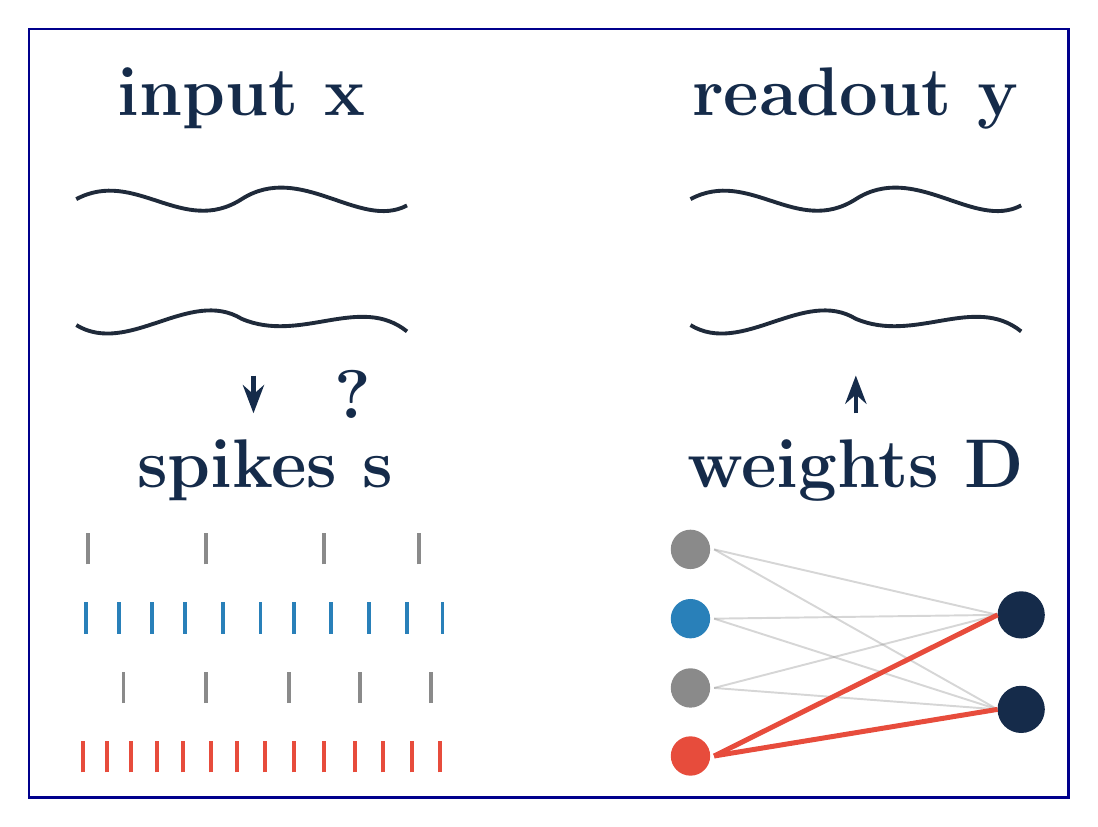
\begin{tikzpicture}[font=\Huge, >=Stealth, x=3.0cm, y=1.6cm]
    % border: 2x2 grid layout
    %   top-left     input x       |  top-right    readout y
    %   bottom-left  spikes s      |  bottom-right weights D
    \draw[accent, line width=1pt, rounded corners=0pt]
        (-0.20, -4.20) rectangle (4.20, 1.90);
    \begin{scope}
      \definecolor{nGr}{HTML}{8A8A8A}
      % Match the two-neuron colors used throughout the poster (B1=red, B2=blue)
      \definecolor{nBl}{HTML}{2980B9}
      \definecolor{nRe}{HTML}{E74C3C}

      % column/row headers, positioned above each panel individually
      \node[font=\Huge\bfseries, navy] at (0.70, 1.35) {input $\xx$};
      \node[font=\Huge\bfseries, navy] at (3.30, 1.35) {readout ${\yy}$};
      \node[font=\Huge\bfseries, navy] at (0.80, -1.60) {spikes $\vv{s}$};
      \node[font=\Huge\bfseries, navy] at (3.30, -1.60) {weights $\DD$};

      % ═══ top-left: input signals (panel 1, shift (0,0)) ═══
      \begin{scope}[shift={(0,0)}]
        \draw[ink, line width=1.4pt]
            (0,0.55) .. controls (0.25,0.80) and (0.45,0.25) ..
            (0.70,0.55) .. controls (0.95,0.85) and (1.20,0.30) .. (1.40,0.50);
        \draw[ink, line width=1.4pt]
            (0,-0.45) .. controls (0.22,-0.70) and (0.48,-0.15) ..
            (0.70,-0.40) .. controls (0.95,-0.60) and (1.20,-0.20) .. (1.40,-0.50);
      \end{scope}

      % --- downward arrow from panel 1 (input) to panel 2 (spikes) ---
      \node[font=\fontsize{34.5}{40}\selectfont\bfseries, anchor=west, navy]
          at (1.05, -1.00) {?};
      \draw[->, navy, line width=1.6pt] (0.75, -0.85) -- (0.75, -1.15);

      % --- upward arrow from panel 3 (weights) to panel 4 (readout) ---
      \draw[->, navy, line width=1.6pt] (3.30, -1.15) -- (3.30, -0.85);

      % ═══ bottom-left: spike raster (panel 2, shift (0,-3.2), 4 rows) ═══
      \begin{scope}[shift={(0,-3.2)}]
        \foreach \t in {0.05,0.55,1.05,1.45}
            \draw[nGr, line width=1.4pt] (\t,0.85) -- (\t,1.10);
        \foreach \t in {0.04,0.18,0.32,0.46,0.62,0.78,0.92,1.08,1.24,1.40,1.55}
            \draw[nBl, line width=1.4pt] (\t,0.30) -- (\t,0.55);
        \foreach \t in {0.20,0.55,0.90,1.20,1.50}
            \draw[nGr, line width=1.4pt] (\t,-0.25) -- (\t,0.00);
        \foreach \t in {0.03,0.13,0.23,0.34,0.45,0.57,0.68,0.80,0.92,1.05,1.18,1.30,1.42,1.54}
            \draw[nRe, line width=1.4pt] (\t,-0.80) -- (\t,-0.55);
      \end{scope}

      % ═══ bottom-right: weights D (panel 3, shift (2.6,-3.2),
      %     4 source dots, 2 readout dots) ═══
      \begin{scope}[shift={(2.6,-3.2)}]
        % absolute-mm radii so dots stay circular under anisotropic x/y units
        \foreach \y/\col in {0.97/nGr,0.42/nBl,-0.13/nGr,-0.67/nRe}
            \fill[\col] (0.00,\y) circle [radius=2.5mm];
        \fill[navy] (1.40,0.45) circle [radius=3mm];
        \fill[navy] (1.40,-0.30) circle [radius=3mm];
        % background decoder weights (faded)
        \foreach \y in {0.97,0.42,-0.13}{
            \draw[nGr, opacity=0.35, line width=0.7pt] (0.10,\y) -- (1.30,0.45);
            \draw[nGr, opacity=0.35, line width=0.7pt] (0.10,\y) -- (1.30,-0.30);}
        % highlighted Di = orange (bottom neuron); same dot size as others
        \draw[nRe, line width=1.8pt] (0.10,-0.67) -- (1.30,0.45);
        \draw[nRe, line width=1.8pt] (0.10,-0.67) -- (1.30,-0.30);
      \end{scope}

      % ═══ top-right: readout signals (panel 4, shift (2.6,0)) ═══
      \begin{scope}[shift={(2.6,0)}]
        \draw[ink, line width=1.4pt]
            (0,0.55) .. controls (0.25,0.80) and (0.45,0.25) ..
            (0.70,0.55) .. controls (0.95,0.85) and (1.20,0.30) .. (1.40,0.50);
        \draw[ink, line width=1.4pt]
            (0,-0.45) .. controls (0.22,-0.70) and (0.48,-0.15) ..
            (0.70,-0.40) .. controls (0.95,-0.60) and (1.20,-0.20) .. (1.40,-0.50);
      \end{scope}
    \end{scope}
\end{tikzpicture}
\end{document}